\section{Outputs}
  In this penultimate section, I will share some of the outputs the project has delivered. I will use these to reflect on the different parts of the project
  each output is associated with. To do this reflection I will use the Experience, Reflect, Action (ESA) framework founded by Melanie Jasper (2003, p.2).

  \begin{figure}[H]
    \centering
    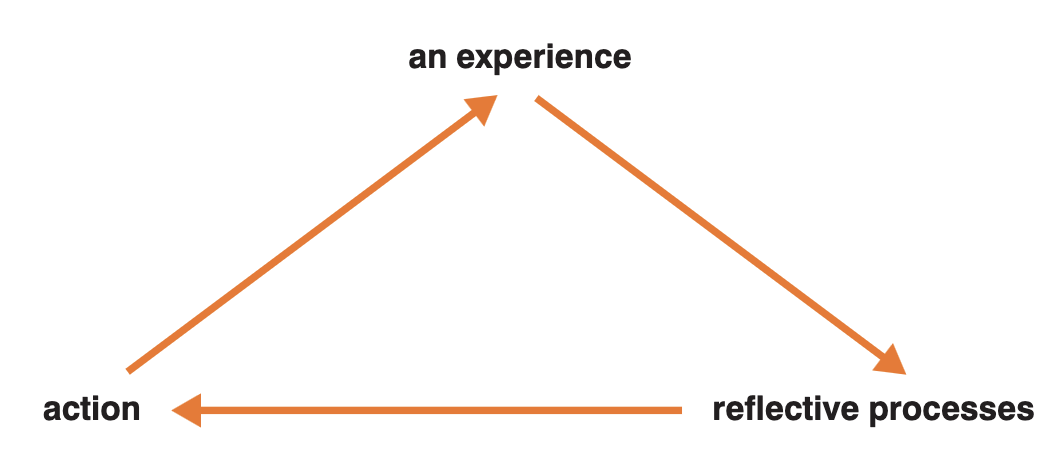
\includegraphics[width=8cm]{assets/eraReflection.png}
    \caption{ERA reflection model founded by Jasper (2003, p.2).}
    \label{fig:eraReflection}
  \end{figure}  

  \subsection{Burn-up Charts}
  \label{sec:burnup}

  \begin{figure}[H]
    \centering
    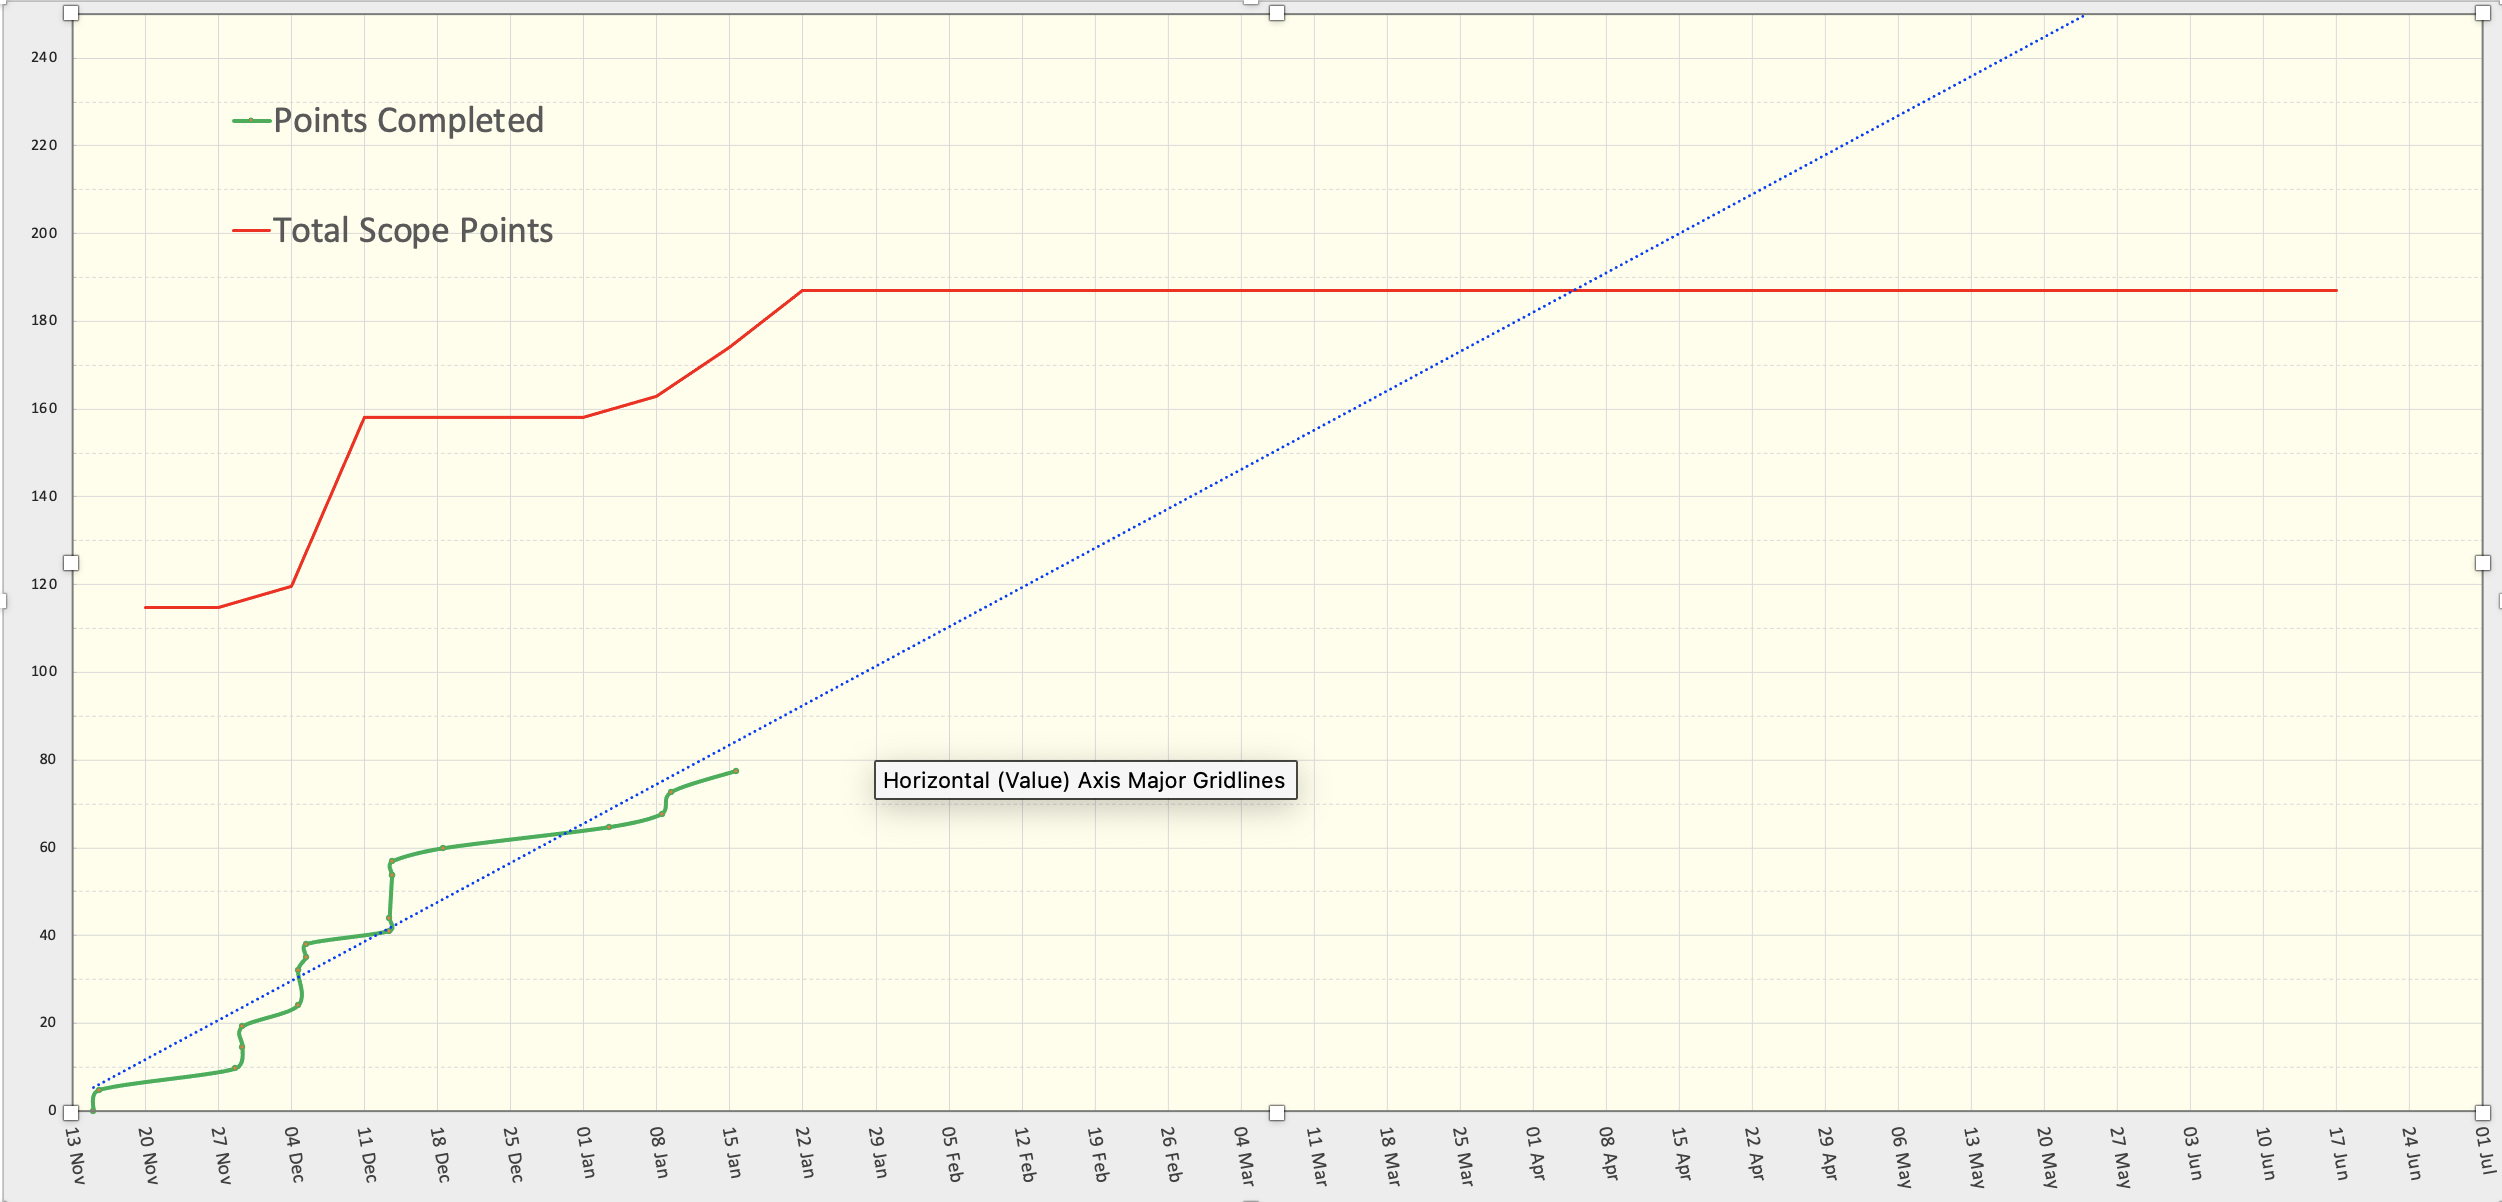
\includegraphics[width=6cm]{assets/outputs/burnups/01-16.png}
    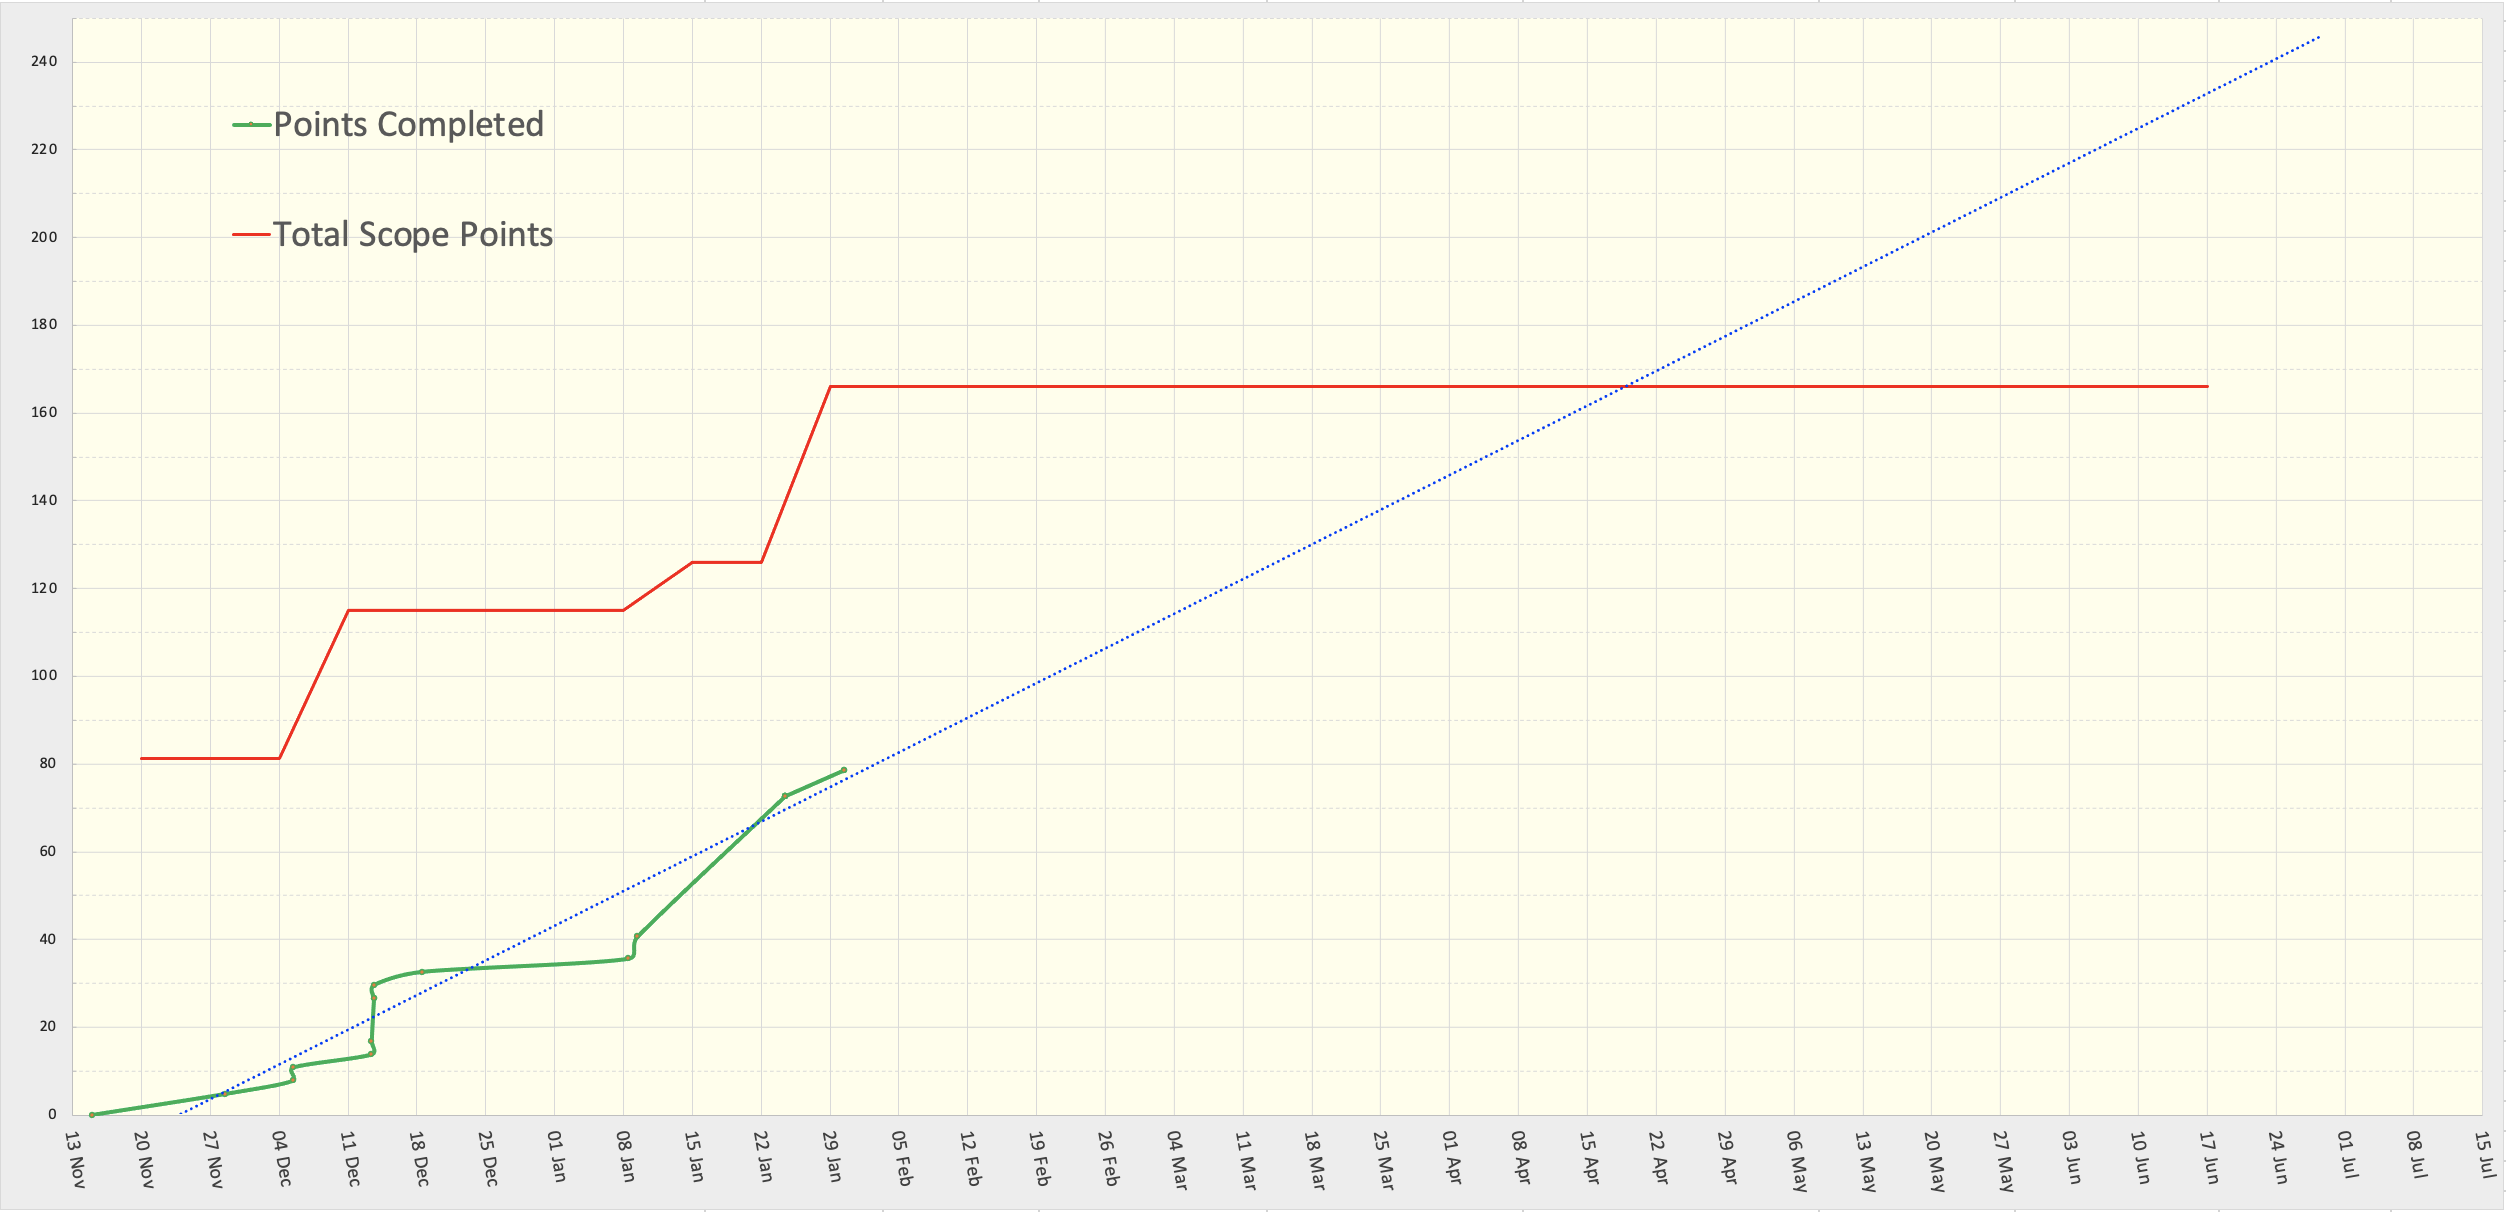
\includegraphics[width=6cm]{assets/outputs/burnups/01-30.png}
    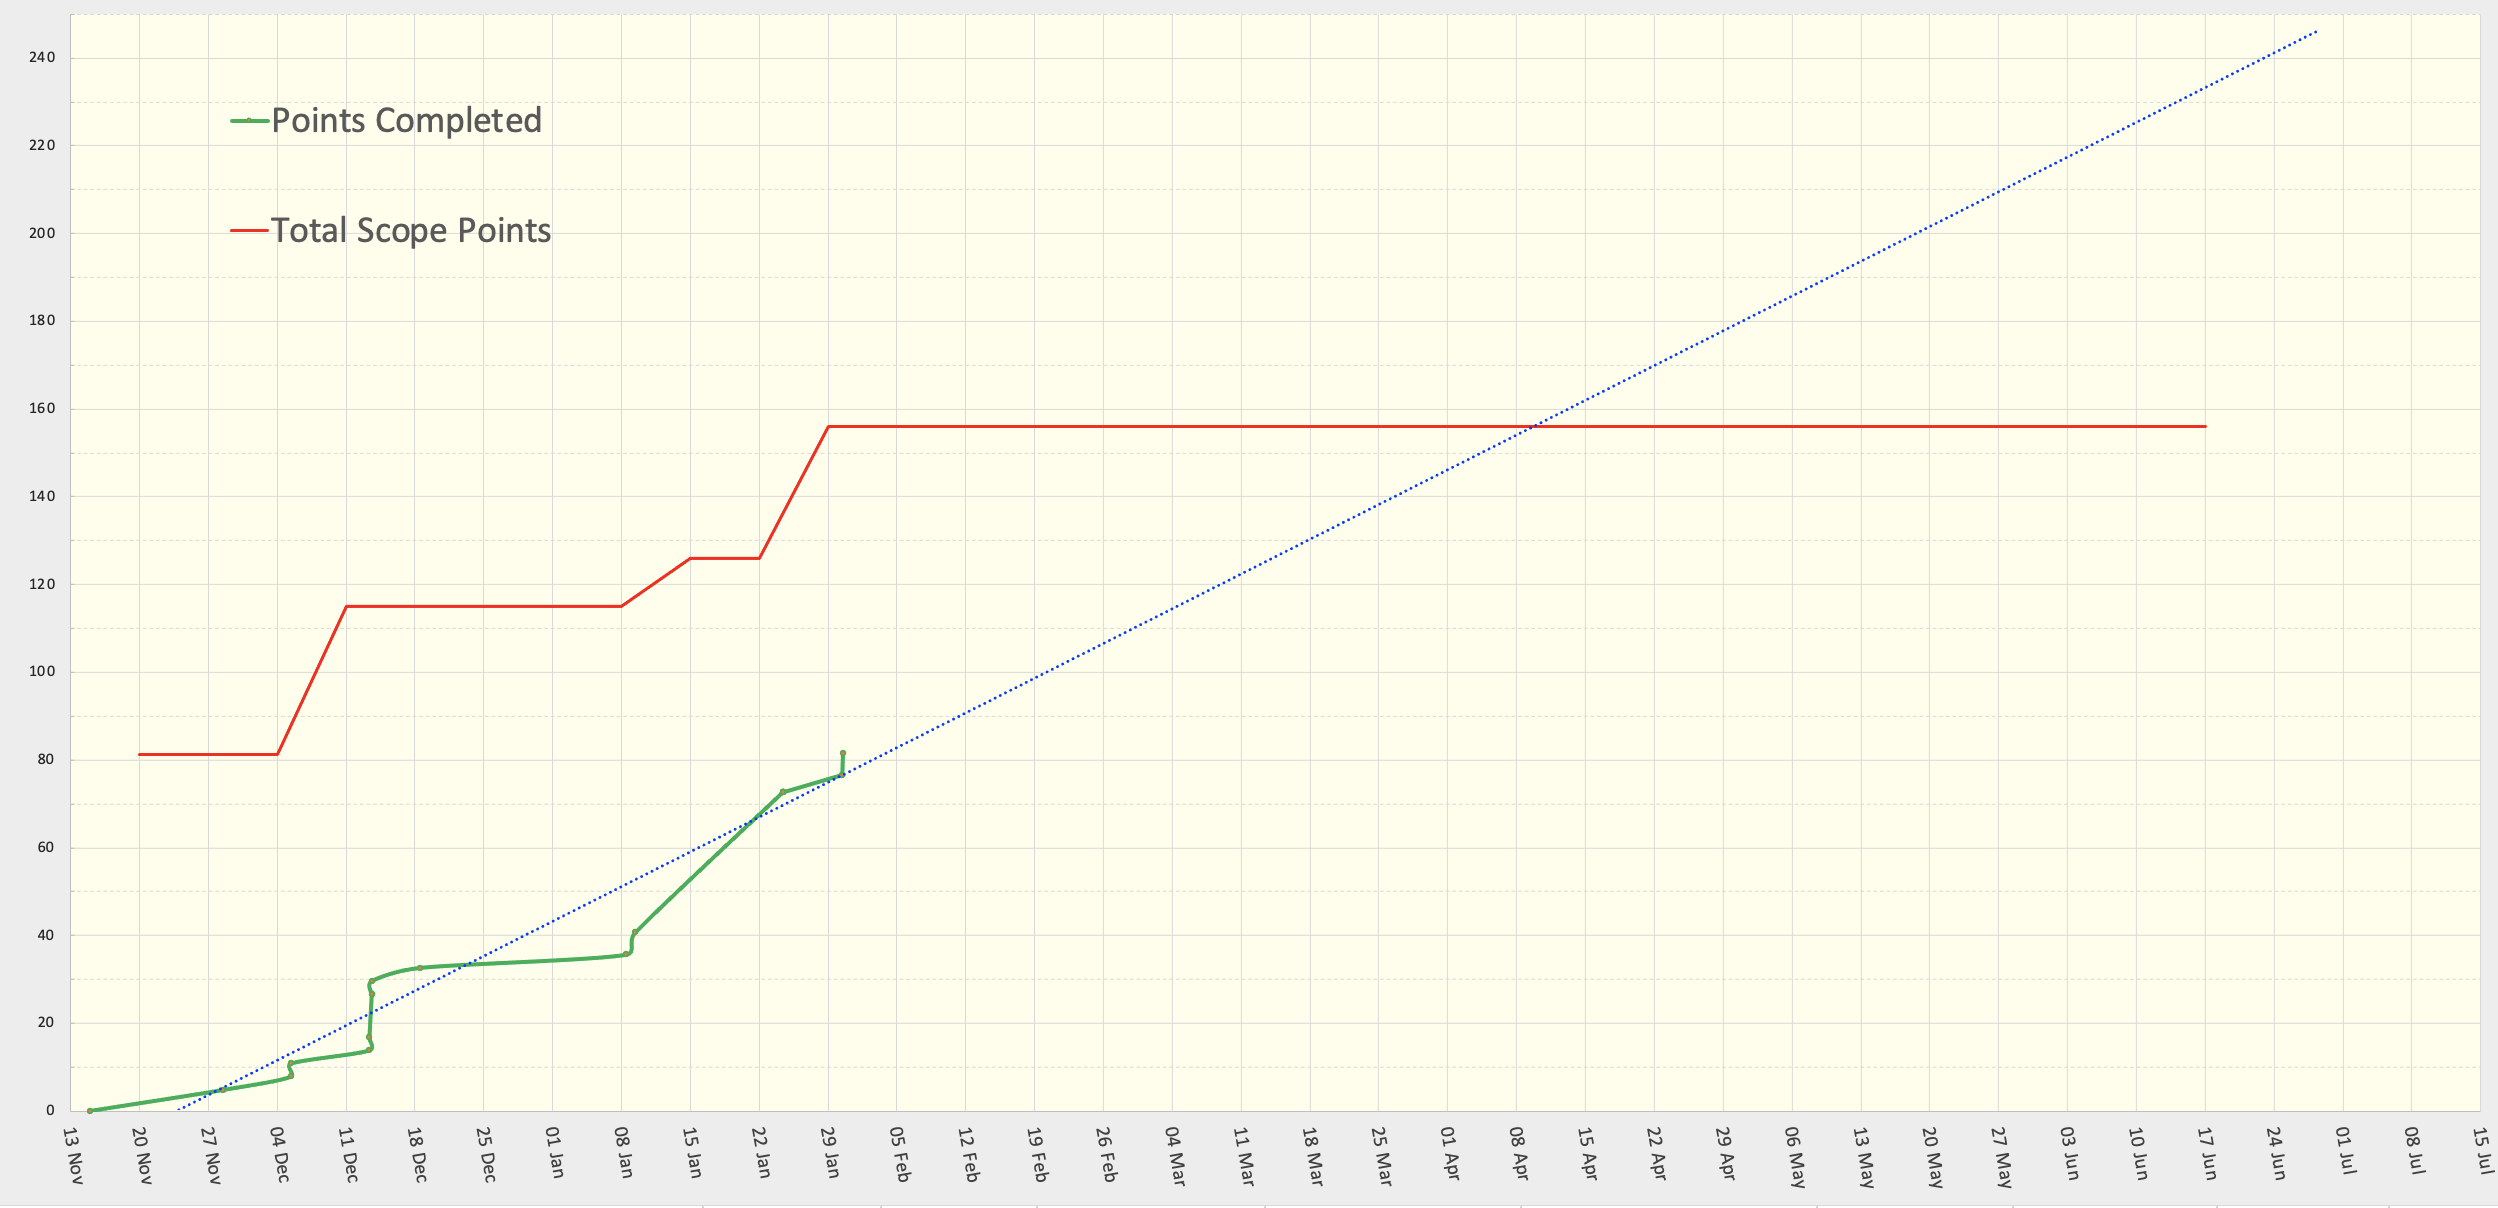
\includegraphics[width=6cm]{assets/outputs/burnups/02-05.png}
    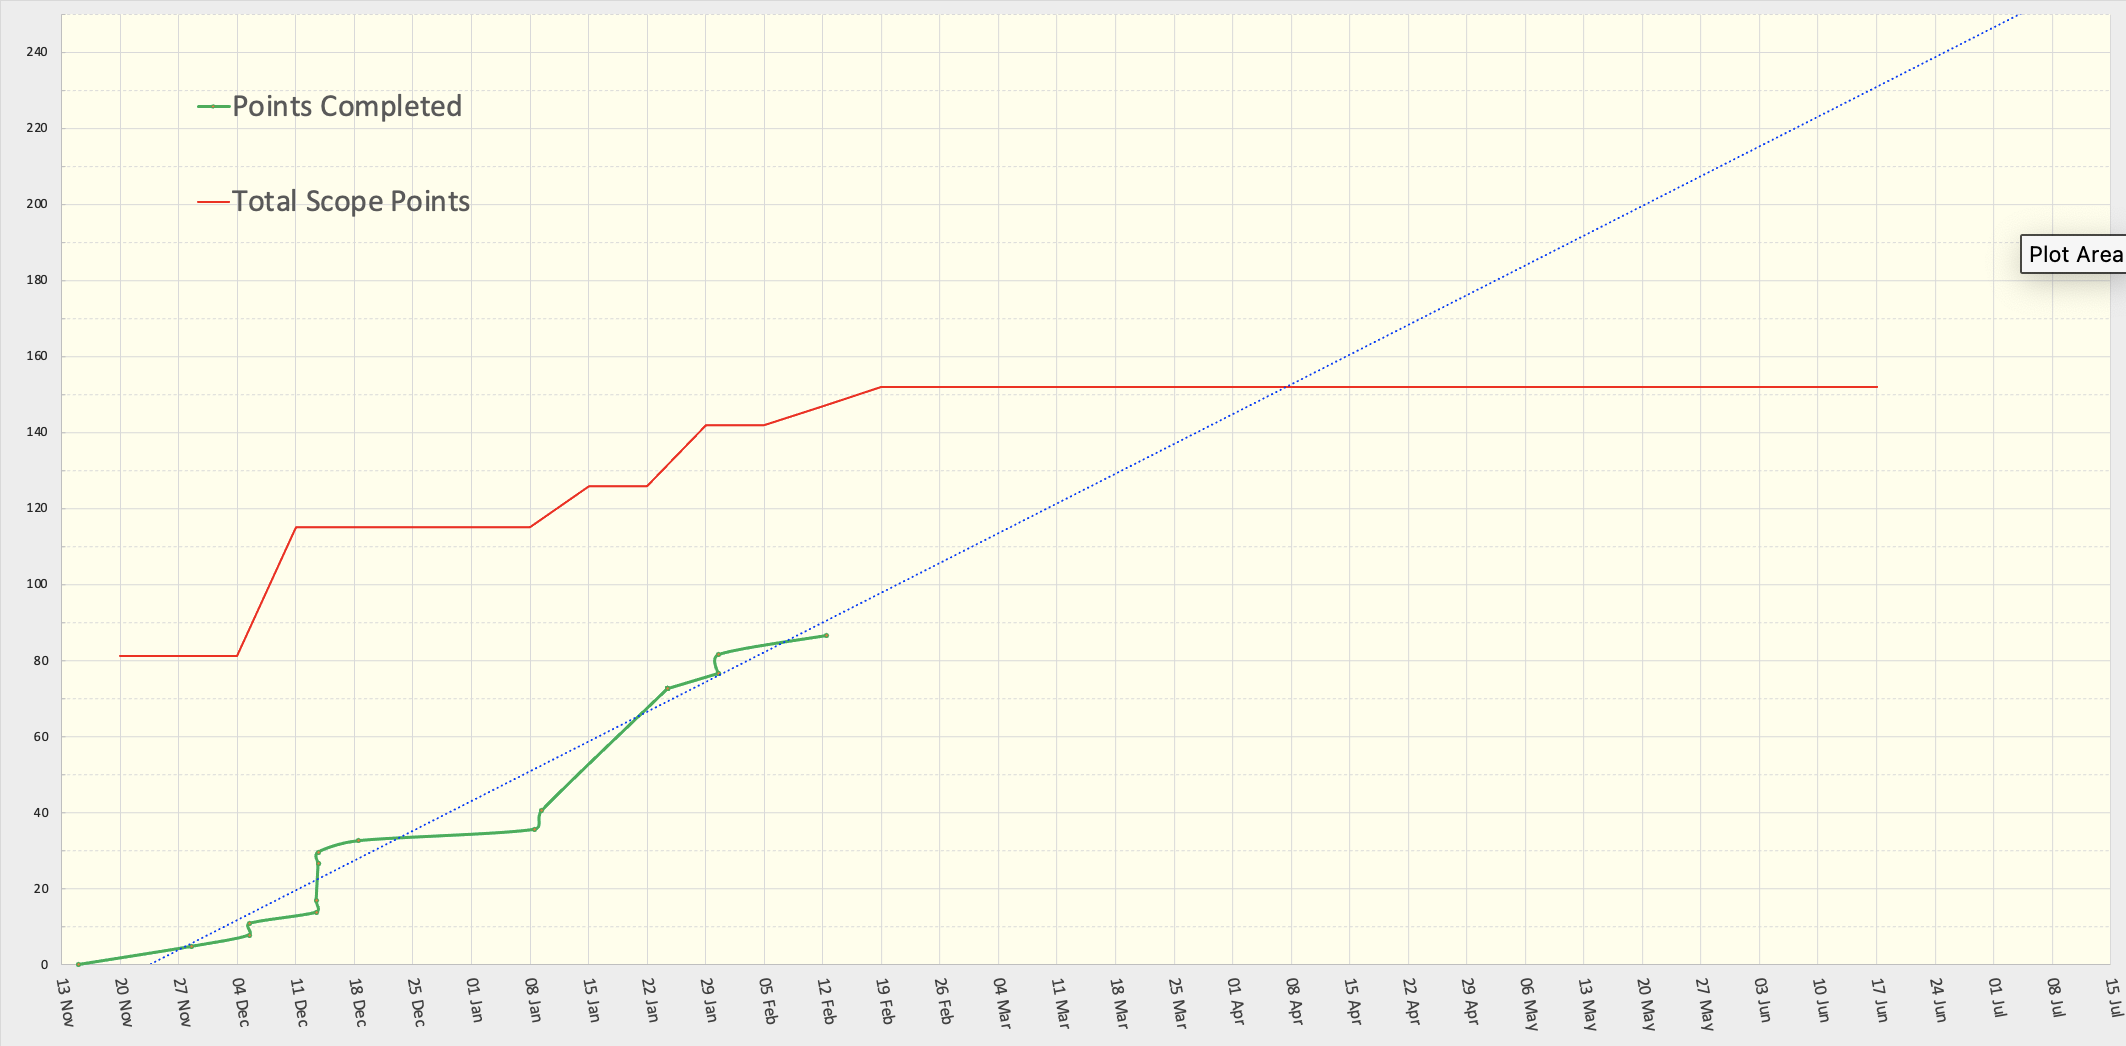
\includegraphics[width=6cm]{assets/outputs/burnups/02-14.png}
    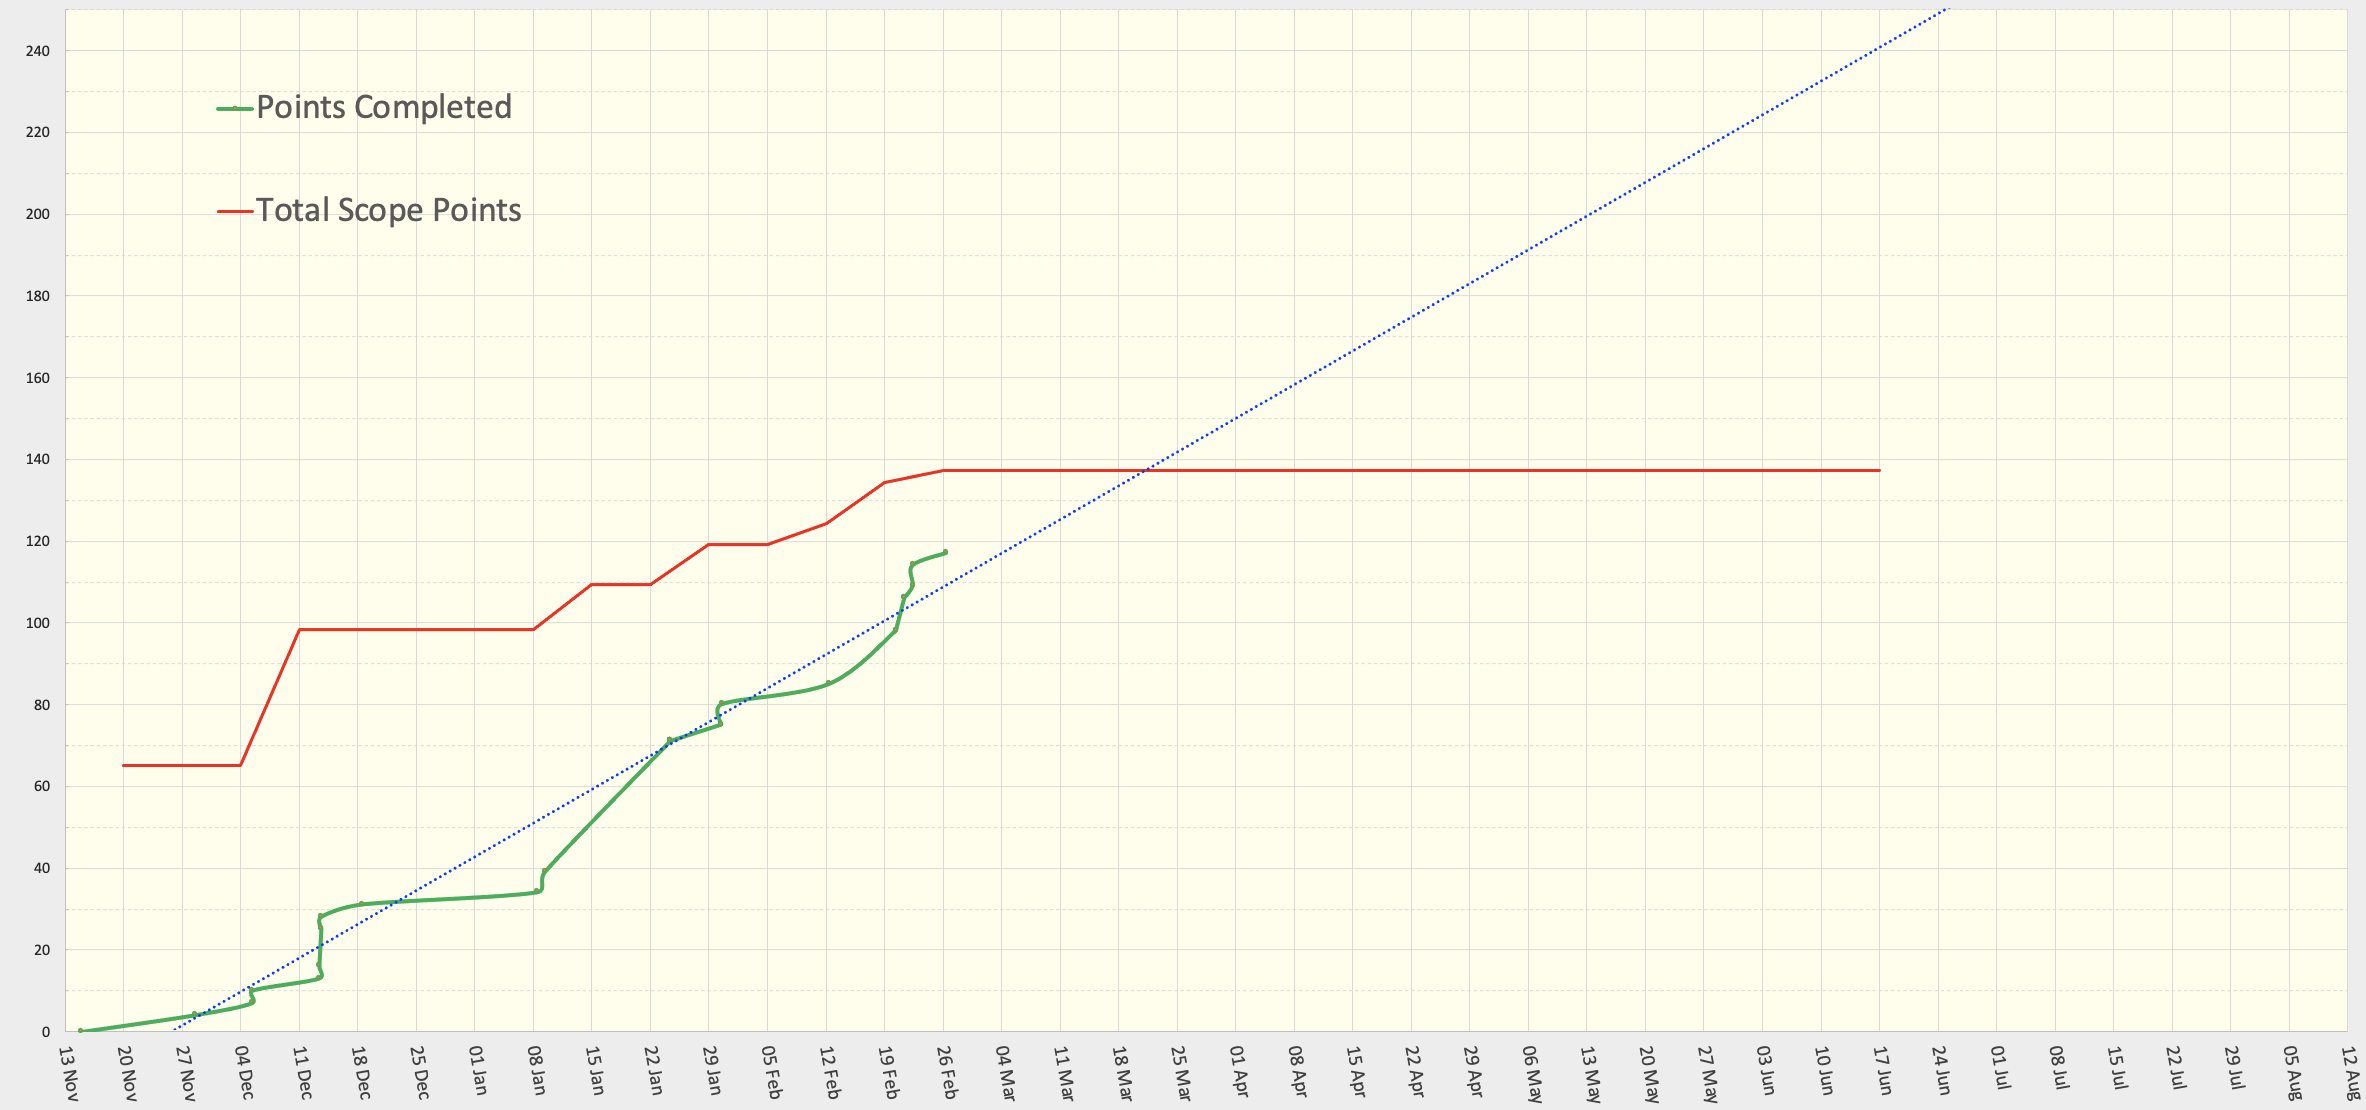
\includegraphics[width=6cm]{assets/outputs/burnups/02-27.png}
    \caption{Burn-up charts throughout the project.}
    \label{fig:burnups}
  \end{figure}

  \textbf{Experience} -
  \textbf{Reflection} -
  \textbf{Action} -

  \newpage
  \subsection{Final System Architecture}

  \textbf{Experience} - 

  \textbf{Reflection} -

  \textbf{Action} -

  \begin{landscape}
    \begin{figure}[H]
      \centering
      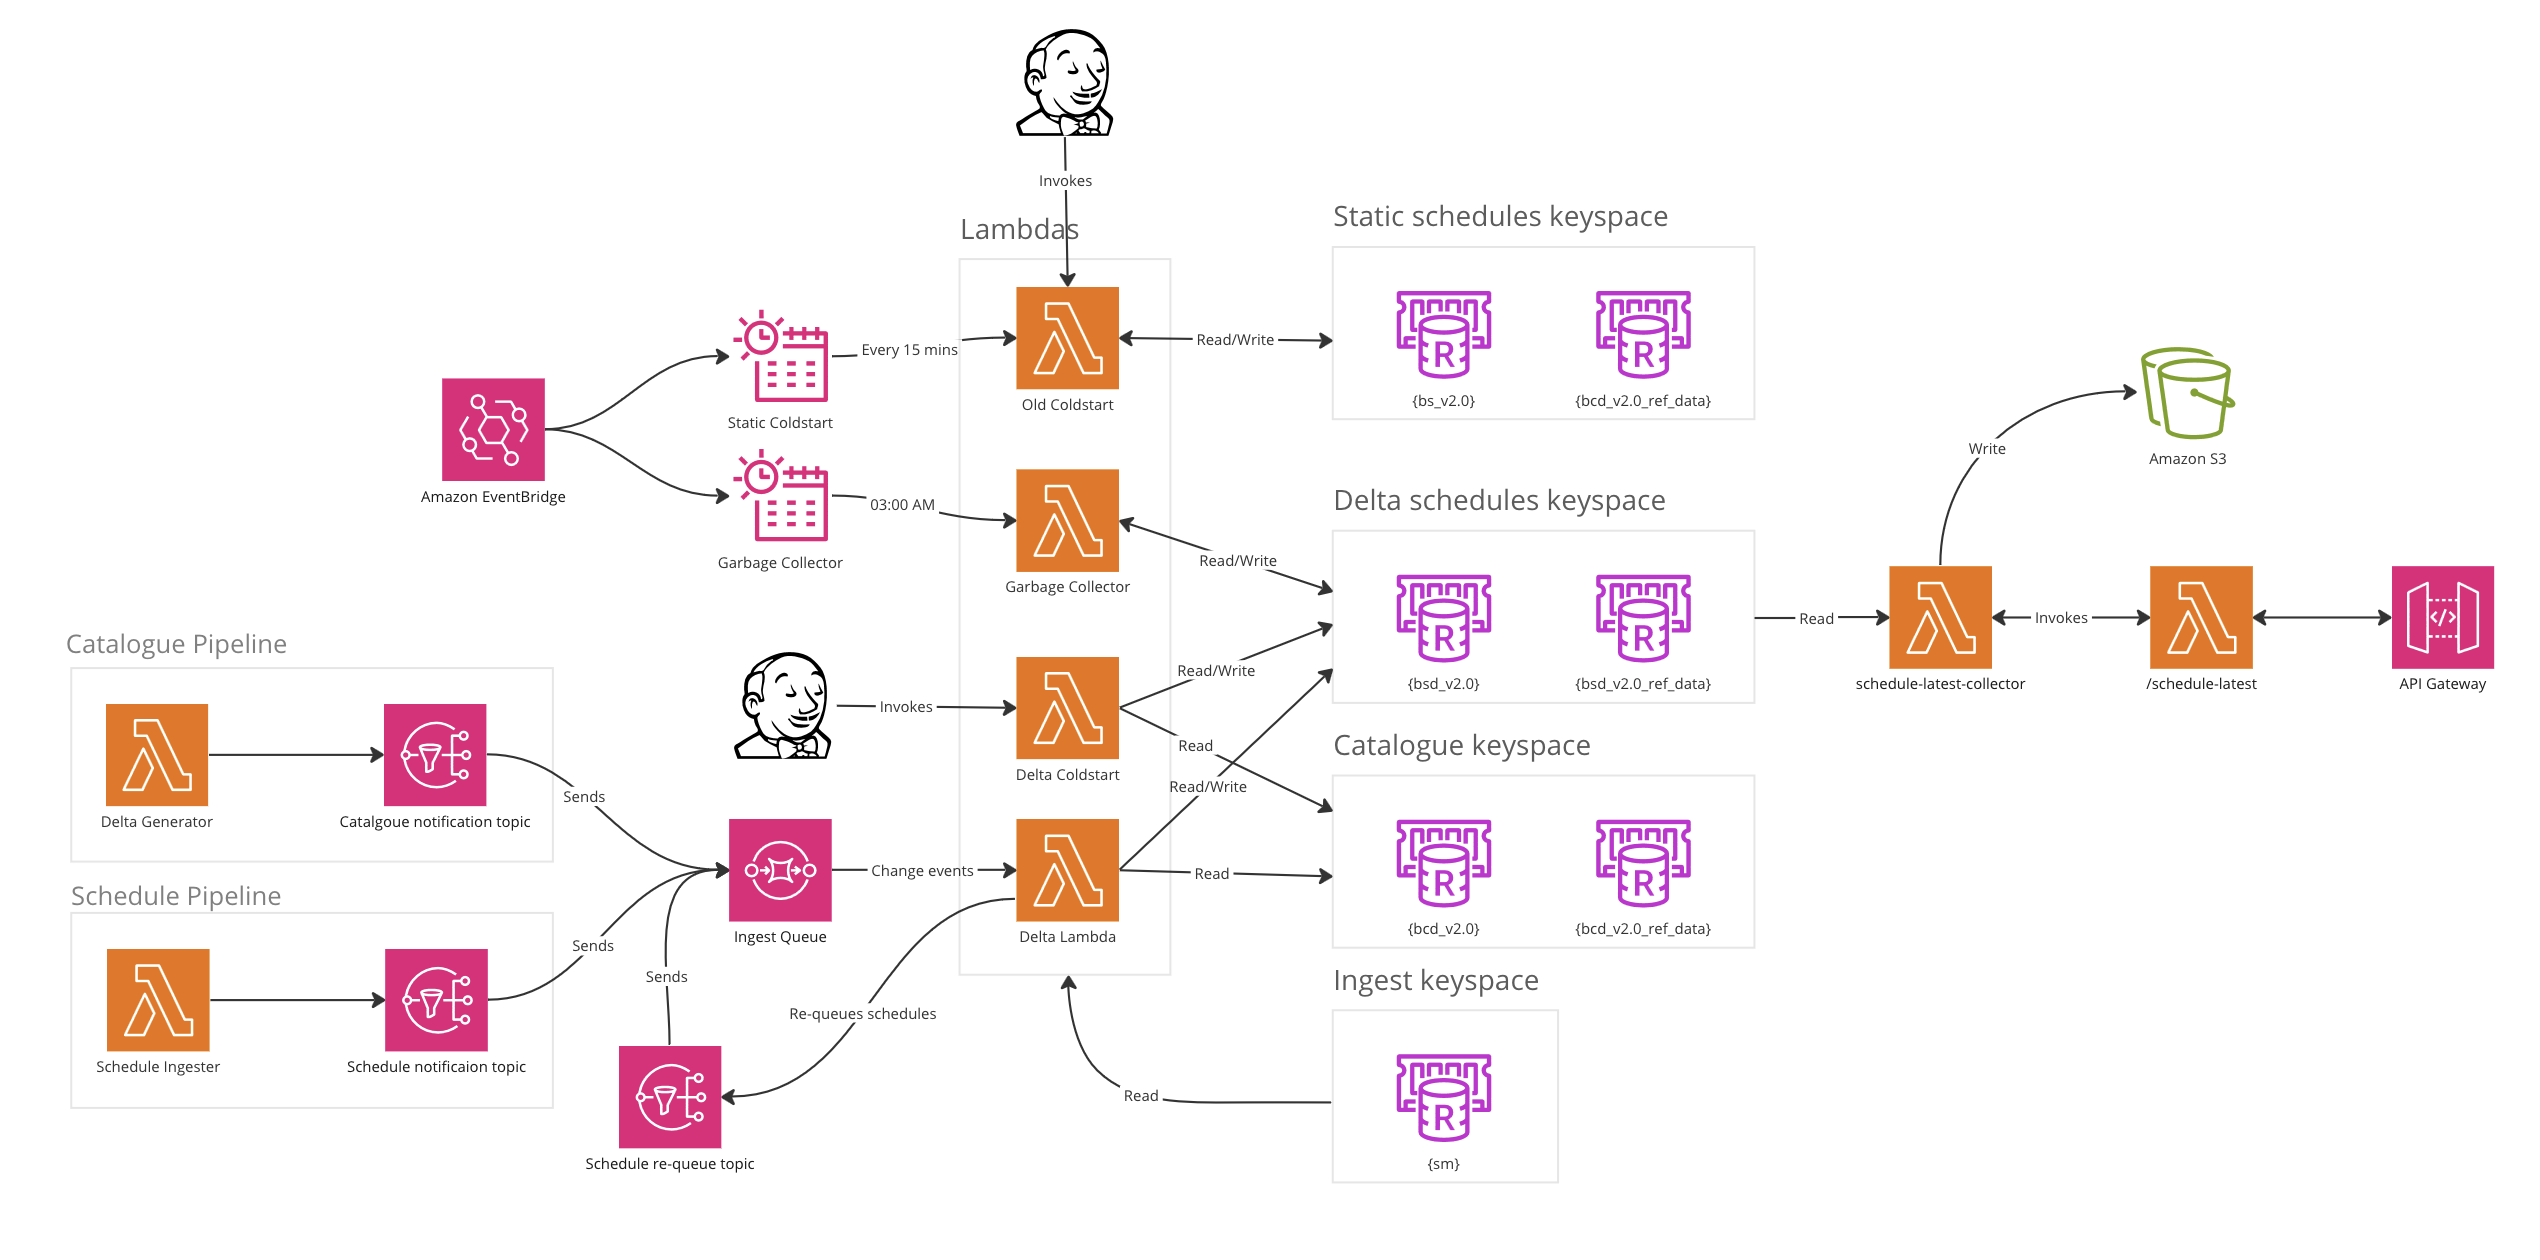
\includegraphics[width=20cm]{assets/outputs/finalArchitecture.png}
      \caption{Final architecture for project.}
      \label{fig:finalArchitecture}
    \end{figure}
  \end{landscape}

  \newpage
  \subsection{Dashboard}

  \textbf{Experience} - Dashboards have been created using a tool called Grafana (2024) that pulls metrics (Amazon Web Services, 2024m) from AWS and
  displays them all in one place. This allows us to check for anomalies and errors. Some metrics such as lambda run-times and invocations are provided by 
  AWS but custom metrics have also been created to track errors, redis writes and schedule re-queues. Metrics are collected during the run time of the 
  lambda using variations of the following code.

   \begin{lstlisting}[caption=Code used to update a metric\, this variation tracks a schedule delete.]
    monitoring.collect({
      typeId: 'Processing',
      result: 'throughput',
      dimensions: {
        ObjType: 'service_schedule',
        EventType: 'Delete'
      },
      value: 1
    })
  \end{lstlisting}

  \textbf{Reflection} - I've used metrics and dashboards throughout my time at the BBC so this is not something that is new to me. Usually the process of 
  adding these metrics is done at the very end of development. This stops monitoring during development which is only a negative. Due to the use of a spike 
  in this project we were able to know what metrics we wanted to track from the start and therefore added them along the way. This helped a lot as metrics on 
  both test and live could be compared to one another as a way to validate that changes had occurred.
  
  \textbf{Action} - Continue to use spikes where necessary and put more thought into what kind of metrics we want to track before development starts.
  This allows comparisons between different dashboards as well as saves one or multiple extra tasks at the end of development to create the metrics and
  dashboards.

  \begin{figure}[H]
    \centering
    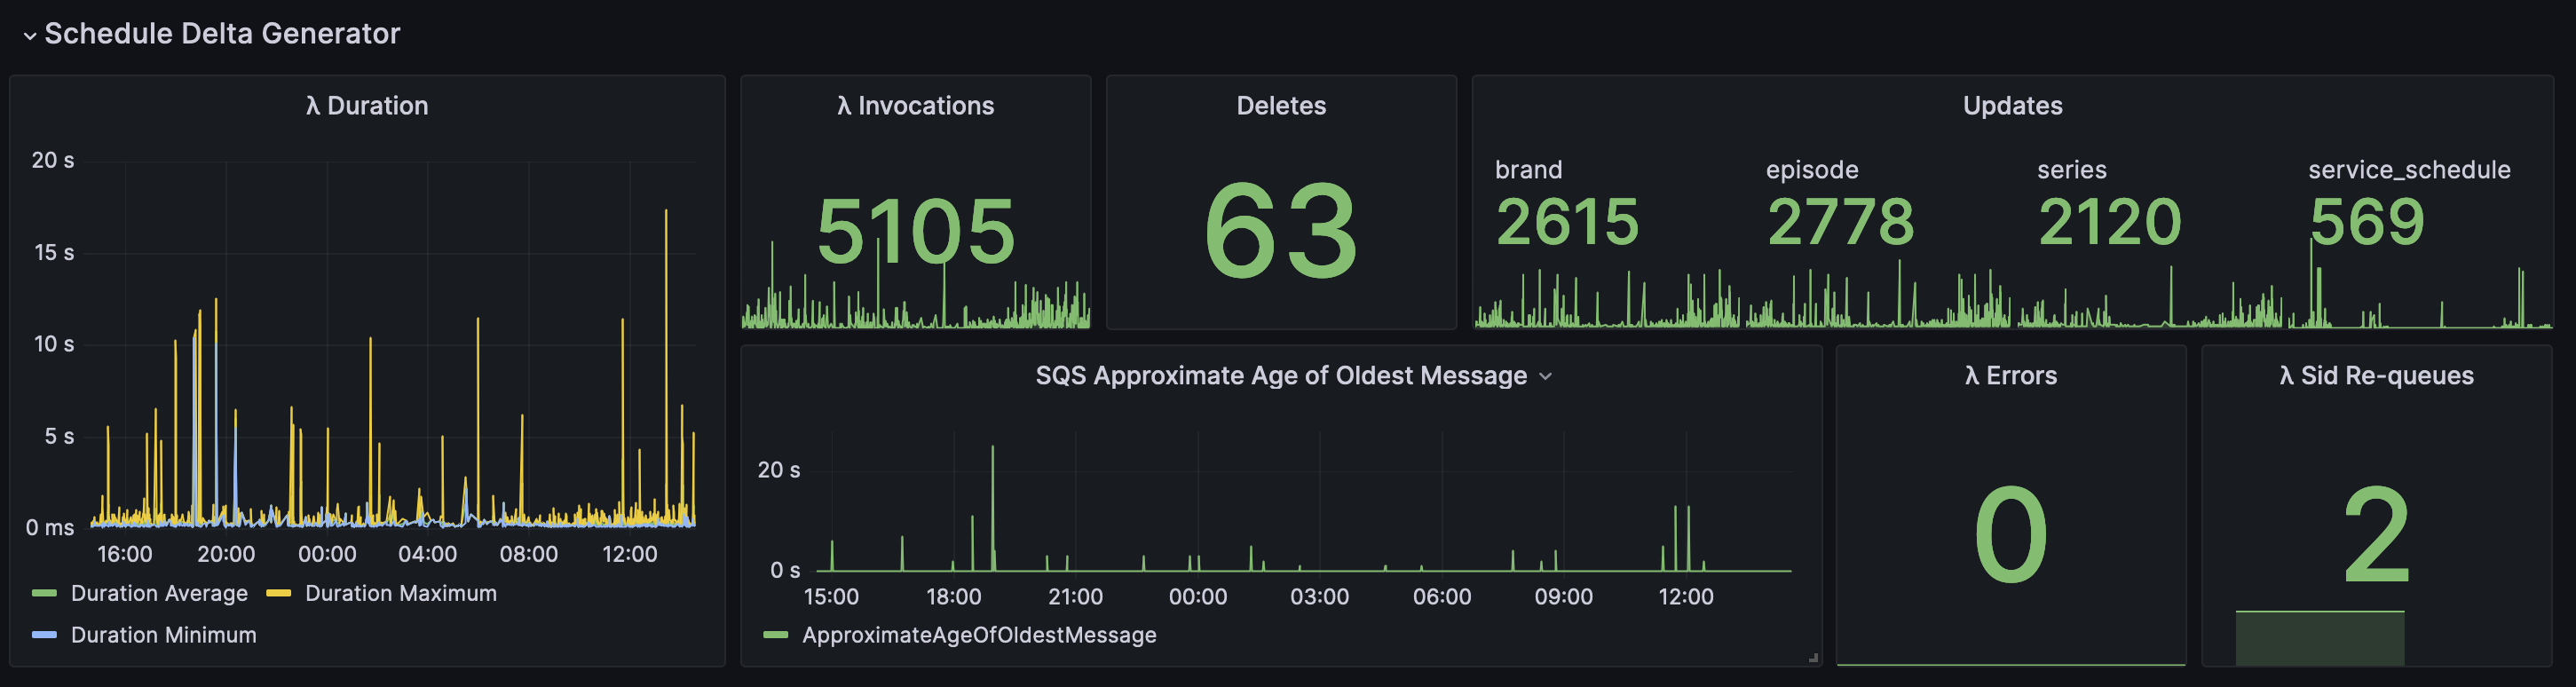
\includegraphics[width=12cm]{assets/outputs/dashboard.png}
    \caption{Created dashboard in Grafana.}
    \label{fig:dashboard}
  \end{figure}
  
  \newpage
  \subsection{Code Base and Commits}

  \begin{figure}[H]
    \centering
    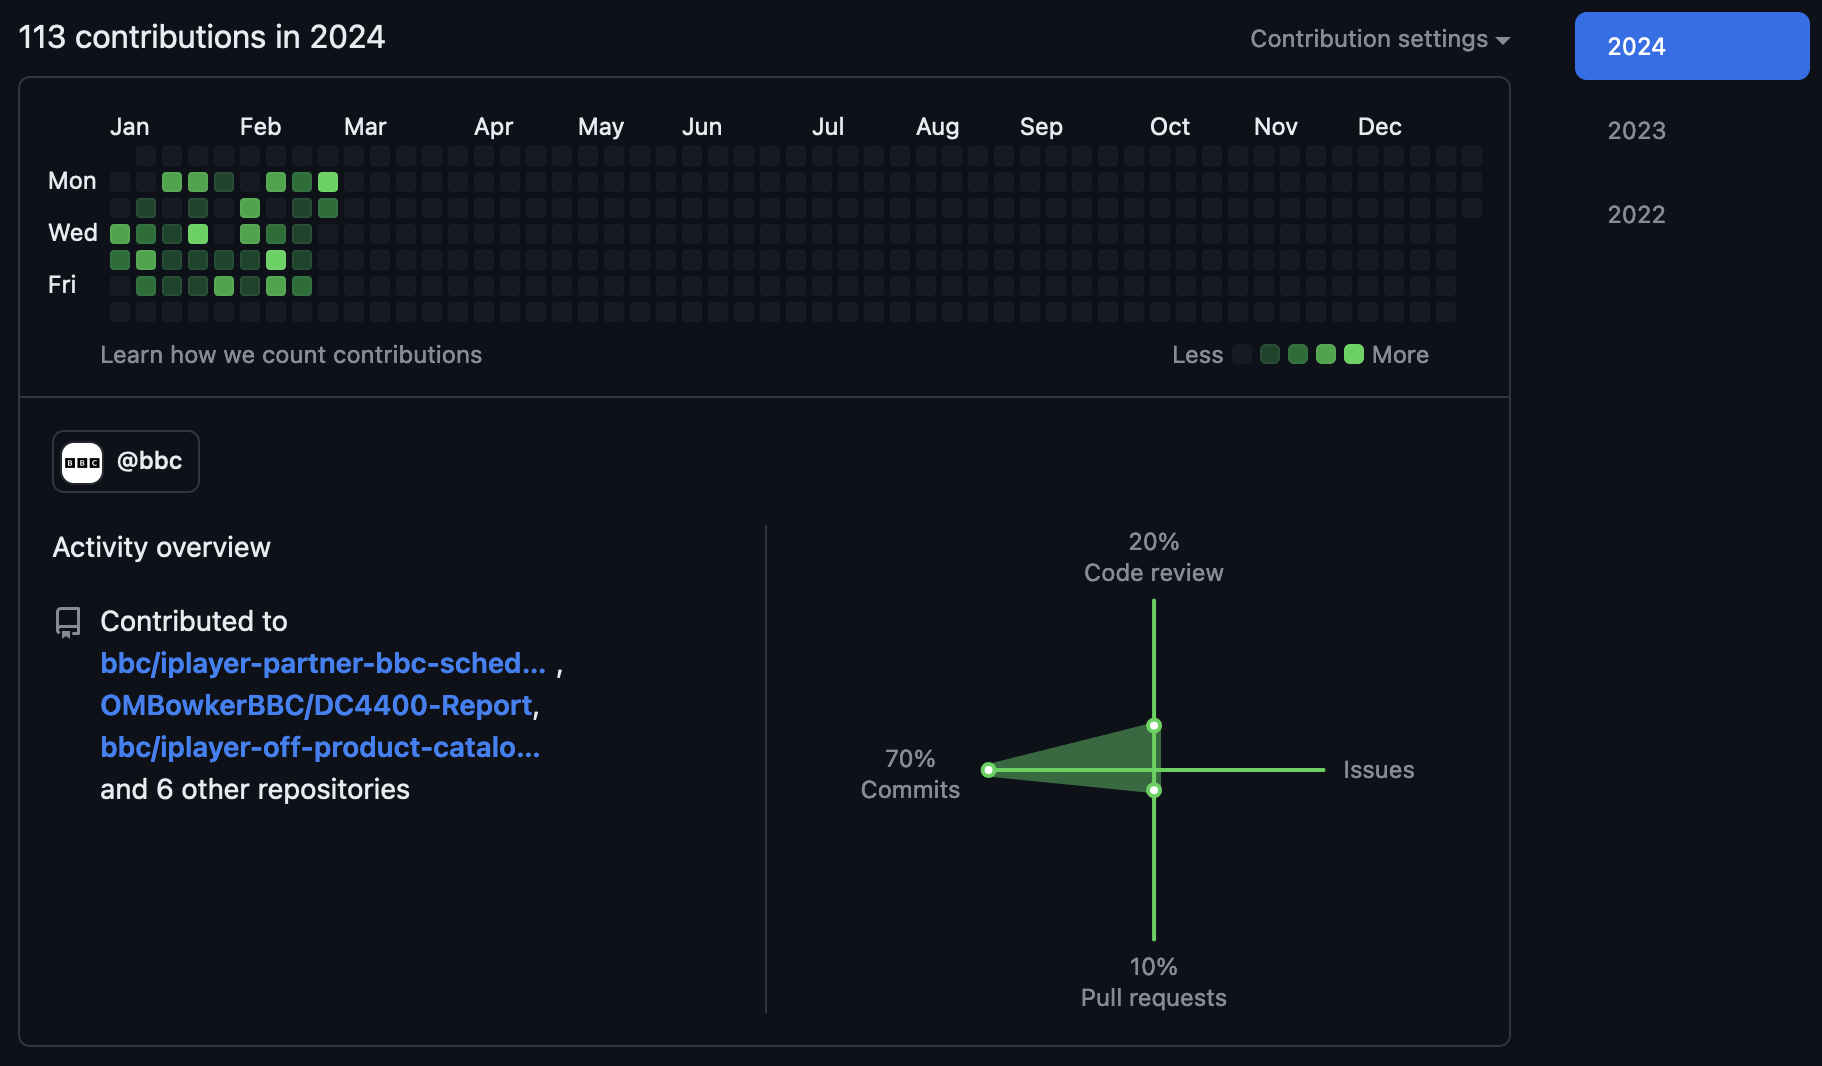
\includegraphics[width=10cm]{assets/outputs/githubContributions.png}
    \caption{Github contributions for my work profile.}
    \label{fig:githubContributions}
  \end{figure}

  \textbf{Experience} -
  \textbf{Reflection} -
  \textbf{Action} -

\newpage
